%===========================
% Chapitre 4 : Valorisation des CDS
%===========================
\chapter{Valorisation des Credit Default Swaps (CDS)}
\label{chap:cds_valuation}

\section{Standardisation et Cotation (Depuis 2009)}

Depuis la standardisation du marché des CDS (le "Big Bang" de 2009), les contrats s'échangent avec un coupon fixe standardisé ($c$) payé par l'acheteur de protection au vendeur :
\begin{itemize}
    \item \textbf{Investment Grade} : coupon $c = 100$ bps ($1\%$)
    \item \textbf{High Yield} : coupon $c = 500$ bps ($5\%$)
\end{itemize}

Puisque le coupon fixe $c$ diffère g\'en\'eralement du spread de marché (par spread $s$), un paiement initial appelé \textbf{Upfront Price} ($UF$) est échangé à l'initiation du contrat pour compenser cette différence. La valeur des deux jambes (au pair vs au coupon standard) doit s'équilibrer :
\begin{equation}
    s \times PV01 = UF + c \times PV01
\end{equation}

Ce qui donne la formule du prix Upfront :
\begin{tcolorbox}[colback=green!5,colframe=green!40!black,title=Upfront Price]
\begin{equation}
    UF = (s - c) \times PV01
\end{equation}
\end{tcolorbox}
Où $PV01$ correspond à la \textit{durée risquée} (Risky Duration), définie comme l'intégrale des probabilités de survie actualisées :
\begin{equation}
    PV01 = \int_{t_0}^T e^{-(r+\lambda)(u-t_0)} du = \frac{1 - e^{-(r+\lambda)(T-t_0)}}{r+\lambda}
\end{equation}

\begin{remarque}[Cotation en Spread vs Contrat en Upfront]
Dans la pratique de marché, bien que les contrats physiques soient standardisés et réglés via l'échange d'un flux \textit{Upfront}, les traders continuent de coter et de négocier les CDS en termes de \textbf{spread} ("live spread"). Le spread reste en effet la métrique la plus intuitive, car elle représente conceptuellement une prime ajoutée à un taux sans risque. La formule ci-dessus permet de passer sans ambiguïté de l'une à l'autre de ces conventions à partir du moment où le coupon standard $c$ est connu.
\end{remarque}

\section{Risques et Sensibilités (DV01)}

Le \textbf{DV01} (Dollar Value of a 01) représente la sensibilité du prix du CDS (son Upfront) à un mouvement du spread de marché $s$ :
\begin{equation}
    DV01 = \frac{\partial UF}{\partial s} = PV01 + (s - c) \times \underbrace{\frac{\partial PV01}{\partial s}}_{< 0}
\end{equation}

\begin{remarque}
Il est important de noter que \textbf{$DV01 \neq PV01$} sauf si l'obligation cote au pair ($s = c$). En effet, la durée risquée elle-même est une fonction décroissante du spread. Une augmentation du spread s'accompagne d'une hausse du risque de défaut (via l'intensité $\lambda$), ce qui réduit l'espérance de la durée de vie des paiements et donc la durée risquée ($\frac{\partial PV01}{\partial s} < 0$).
\end{remarque}

\section{Intensité de Défaut et Recouvrement}

Dans ce modèle, l'intensité de défaut implicite $\lambda$ est extraite du marché via la relation d'absence d'opportunité d'arbitrage (AOA) :
\begin{equation}
    \lambda = \frac{s}{1 - R}
\end{equation}
Le taux de recouvrement $R$ est généralement supposé constant pour les calculs de valorisation. Sa valeur standard dépend de la séniorité de la dette de l'entité de référence :
\begin{itemize}
    \item \textbf{Senior Unsecured CDS} : $R = 40\%$
    \item \textbf{Subordinated CDS} : $R = 20\%$
\end{itemize}

\section{En pratique : Le Modèle Standard ISDA}

\subsection{Calibrage des Probabilités de Survie}

En pratique, les probabilités de survie $S(t)$ sont calibrées sur les prix des CDS liquides du marché pour les maturités standards (\textit{tenors}) : \textbf{1Y, 2Y, 3Y, 5Y, 7Y, 10Y}.

Cette construction est réalisée par une méthode de \textbf{bootstrap} (de proche en proche), très similaire à celle utilisée pour la construction des courbes de taux d'intérêt. Elle permet d'estimer et calibrer une courbe de probabilités de survie où l'intensité de défaut $\lambda(t)$ n'est plus supposée constante, mais varie (constante par morceaux) entre chaque maturité.

\subsection{ISDA Standard Model}

L'ISDA (International Swaps and Derivatives Association) a établi un modèle standard (ISDA Standard Model) qui fait référence pour ces valorisations et sépare clairement les deux composantes :

\begin{enumerate}
    \item \textbf{Courbe d'actualisation (Discount Factor)} :
    \begin{equation}
        DF(t) = e^{-\int_0^t r(u) du}
    \end{equation}
    Ce facteur d'actualisation est calibré à partir des taux sans risque du marché interbancaire (\textit{money market} et \textit{swap rates}).
    
    \item \textbf{Courbe de survie (Survival Probability)} :
    \begin{equation}
        S(t) = e^{-\int_0^t \lambda(u) du}
    \end{equation}
    Cette probabilité est calibrée à partir des prix (spreads) des CDS directement sur le marché.
\end{enumerate}

\section{Indices de Crédit}

Le marché du crédit s'appuie fortement sur des indices qui regroupent les CDS des entreprises les plus liquides. Au-delà des spécialistes du crédit, ces indices sont très suivis sur l'ensemble des marchés financiers (formant des indicateurs \textit{cross-asset}) car ils constituent un baromètre macroéconomique direct du risque de crédit. 

On les compare très fréquemment au \textbf{VIX} (l'indicateur de volatilité du S\&P 500 pour le marché Actions) : en cas de krach boursier ou de forte incertitude, ces deux indicateurs sont extrêmement corrélés et "spikent" (augmentent brutalement) de manière simultanée.

\subsection{Fonctionnement des Indices}

\begin{itemize}
    \item \textbf{Deux grandes familles} :
    \begin{itemize}
        \item \textbf{CDX} pour l'Amérique du Nord (NA) et les Marchés Émergents (EM).
        \item \textbf{iTraxx} pour l'Europe.
    \end{itemize}
    \item \textbf{Roulement (Roll)} : Les indices sont mis à jour et "rollés" tous les \textbf{6 mois}, en mars et septembre.
    \item \textbf{Liquidité} : L'essentiel de la liquidité se concentre sur les contrats de maturité \textbf{5 ans (5Y)}.
\end{itemize}

\subsection{Composition (Séries Actuelles)}

La composition, c'est-à-dire la sélection du panier, varie selon la région, la notation (\textit{Rating}) et la séniorité de la dette.

\begin{table}[H]
    \centering
    \begin{tabular}{|l|c|c|c|c|}
        \hline
        \textbf{Index} & \textbf{Region} & \textbf{Rating} & \textbf{Séniorité} & \textbf{Nb de constituants} \\ \hline
        \textbf{CDX IG} & NA & IG & Senior Unsecured & 125 \\ \hline
        \textbf{CDX HY} & NA & HY & Senior Unsecured & 100 \\ \hline
        \textbf{iTraxx Main} & Europe & IG & Senior Unsecured & 125 \\ \hline
        \textbf{iTraxx X-Over} & Europe & HY (Cross-over) & Senior Unsecured & 75 \\ \hline
        \textbf{iTraxx Senior Fin} & Europe & IG & Senior & 30 \\ \hline
        \textbf{iTraxx Sub Fin} & Europe & IG & Subordinated & 30 \\ \hline
    \end{tabular}
    \caption{Principaux indices de crédit et leurs caractéristiques d'après le Modèle Standard}
\end{table}

\begin{remarque}
Rappelons que la séniorité impacte directement l'hypothèse de taux de recouvrement ($R$) utilisé pour calculer le spread $S = \lambda \times (1-R)$ :
\begin{itemize}
    \item Dette \textit{Senior Unsecured} : $R_{SU} = 40\%$
    \item Dette \textit{Subordinated} : $R_{Sub} = 20\%$
\end{itemize}
\end{remarque}

\subsection{Stratégies de Valeur Relative (Relative Value)}

La segmentation des indices \textit{Senior} et \textit{Subordinated} sur les mêmes entités de référence (cas typique des indices iTraxx Financials) permet d'élaborer des stratégies de valeur relative (arbitrage). En effet, pour un même sous-jacent bancaire, l'intensité de défaut $\lambda$ est identique dans les deux contrats. Seul le taux de recouvrement postulé varie.
Ainsi, le rapport théorique d'équilibre (la \textit{Fair Value}) entre les spreads s'écrit :
\begin{equation}
    \frac{Spread_{Sub}}{Spread_{Senior}} = \frac{\lambda \times (1 - R_{Sub})}{\lambda \times (1 - R_{SU})} = \frac{1 - 0.20}{1 - 0.40} = \frac{0.80}{0.60} = \frac{4}{3} \approx 1.33
\end{equation}
\textbf{Trading Long/Short} : Si sur le marché, le ratio observé s'écarte significativement de ce niveau théorique de $\frac{4}{3}$ (légèrement ajusté car certains indices subordonnés incluent des dettes de type \textit{contingent capital} dont le recouvrement est encore plus faible), les \textit{CDS Traders} peuvent initier des opérations de \textbf{Valeur Relative (Relative Value)} : ils se positionnent \textit{Long} sur la protection d'un indice et \textit{Short} sur l'autre, afin de profiter d'un retour à la moyenne historique des écarts de spreads.

\subsubsection{Mise en pratique : Analyse du Ratio et Z-Score}

En pratique, on suit l'évolution du ratio observé sur le marché à l'instant $t$ :
\begin{equation}
    \alpha_t = \frac{S_{\text{Sub}}(t)}{S_{\text{Sen}}(t)}
\end{equation}

Pour quantifier l'ampleur de la déviation par rapport à la moyenne historique $\bar{\alpha}$ (qui gravite autour de $4/3$), l'analyste quantitatif calcule un indicateur statistique centré réduit, le \textbf{Z-Score} :
\begin{equation}
    Z_t = \frac{\alpha_t - \bar{\alpha}}{\sigma(\alpha)}
\end{equation}
où $\sigma(\alpha)$ est l'écart-type historique du ratio $\alpha$.

\begin{figure}[H]
    \centering
    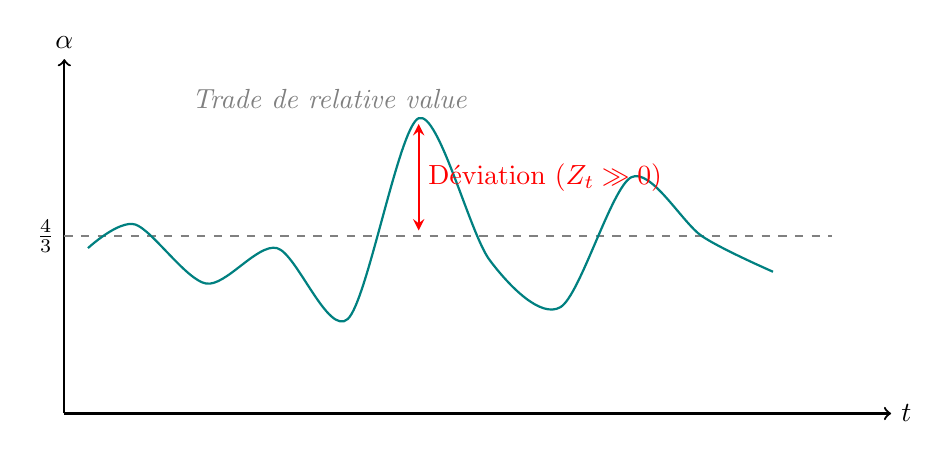
\begin{tikzpicture}[scale=1.5]
        % Axes
        \draw[->, thick] (0,0) -- (7,0) node[right] {$t$};
        \draw[->, thick] (0,0) -- (0,3) node[above] {$\alpha$};
        
        % Ligne theorique (Fair Value)
        \draw[dashed, thick, gray] (0,1.5) -- (6.5,1.5);
        \node[left] at (0,1.5) {$\frac{4}{3}$};
        
        % Courbe du ratio (fluctuations)
        \draw[thick, teal, smooth] plot coordinates {
            (0.2, 1.4) (0.6, 1.6) (1.2, 1.1) (1.8, 1.4) (2.4, 0.8) 
            (3.0, 2.5) (3.6, 1.3) (4.2, 0.9) (4.8, 2.0) (5.4, 1.5) (6.0, 1.2)
        };
        
        % Fleche montrant la deviation
        \draw[<->, >=stealth, thick, red] (3.0, 1.55) -- (3.0, 2.45);
        \node[right, red] at (3.0, 2.0) {Déviation ($Z_t \gg 0$)};
        
        % Titre dans le graphe
        \node[above right, text=gray] at (1, 2.5) {\textit{Trade de relative value}};
    \end{tikzpicture}
    \caption{Évolution du ratio $\alpha_t$ et signal d'arbitrage (Z-Score)}
\end{figure}

Lorsque le Z-Score atteint des valeurs extrêmes (ex: $Z_t \gg 0$), cela signifie que le spread subordonné est "trop large" ou "trop cher" par rapport au spread senior. Le trader anticipe alors une compression de ce ratio.

L'opération d'arbitrage correspondante (Exemple : \textit{Sub vs Sen Fin}) se construit ainsi :
\begin{enumerate}
    \item \textbf{Vente de protection} sur le sous-jacent Subordonné (\textit{Sub Fin}) : on s'expose au risque, espérant que le spread va se resserrer.
    \item \textbf{Achat de protection} sur le sous-jacent Senior (\textit{Sen Fin}) : on se couvre contre un écartement macroéconomique global du secteur financier.
\end{enumerate}

Pour que la position soit immunisée contre les petits mouvements parallèles des spreads (neutre en risque de base ou \textit{spread duration}), les montants notionnels engagés doivent être pondérés par le facteur d'équilibre $\beta = \frac{4}{3}$. La variation de sensibilité de la position s'approxime alors par :
\begin{equation}
    \text{Sensibilité} \approx \Delta I_{\text{Sub}} - \beta \times \Delta I_{\text{Sen}}
\end{equation}

\section{Modélisation Statistique et Élargissement de l'Univers}

Au-delà des relations pures d'arbitrage structurel (comme entre \textit{Senior} et \textit{Subordinated} de la même entité), les équipes de stratégies quantitatives ont développé des modèles pour identifier de nouvelles opportunités de Valeur Relative (RV) systématique sur un univers de CDS individuels beaucoup plus vaste.

\subsection{Le modèle de Fair Value (Juste Valeur) Individuel}

Une approche courante consiste à estimer la valeur théorique (Fair Value) du CDS d'une entreprise à partir de ses données fondamentales :
\begin{itemize}
    \item \textbf{Sélection des variables} : Avec l'essor du \textit{Machine Learning}, il faut isoler les facteurs les plus explicatifs. Des critères statistiques comme l'\textbf{AIC} (Akaike Information Criterion) permettent d'éviter le surapprentissage en pénalisant les modèles trop complexes.
    \item \textbf{Modèles Additifs Généralisés (GAM)} : Ces modèles non-linéaires capturent mieux la réalité que les régressions simples. Dans un exemple classique (modèle SG en 2010), la \textit{Fair Value} du CDS s'expliquait très efficacement avec 3 variables clés : la marge bénéficiaire (\textit{Profit Margin}), le \textbf{levier} (la donnée la plus importante, rappelant l'intuition de Merton), et le fonds de roulement (\textit{Working Capital}).
\end{itemize}
Un spread observé au-dessus de ce prix modélisé signale un CDS historiquement "trop cher" (candidat à la vente de protection si la divergence est liée au bruit de marché).

\subsection{L'impact du Risque Macroéconomique et Souverain}

La robustesse temporelle de ces modèles est cependant mise au défi par les changements de \textit{régime de marché}. Lors de la \textbf{crise de la dette européenne (2011)}, les risques souverains (des pays dits "périphériques" comme l'Italie, l'Espagne, la Grèce) ont supplanté les risques propres aux bilans.

Le modèle purement corrélé à la qualité idiosyncratique de l'entreprise s'effondre lorsque le véritable risque devient systémique (ex: \textit{utilities} ou télécoms lourdement exposés à l'État). 
Seule l'inclusion d'\textbf{une variable macroéconomique reflétant le risque de spread souverain local} dans le modèle de valorisation (Fair Value) a permis de rétablir les performances. Cette observation illustre que la pureté d'une métrique d'évaluation passe par une bonne spécification des risques couverts, afin d'éviter le "bruit exogène" de la crise qui force des déviations qui ne sont pas de simples anomalies statistiques.

\subsection{Systématique Cross-CDS : Clustering et Cointégration}

Construire des trades relatifs empiriques \textit{Pair Trading} $A \leftrightarrow B$ parmi les indices majeurs (250 composants IG) génère plus de $31\,000$ croisements. Ce "bruit combinatoire" exige un double filtrage puissant :

\begin{enumerate}
    \item \textbf{Clustering par proximité de flux} : Regrouper algorithmiquement les crédits dont les \textbf{rendements de spreads (mesurés en hebdomadaire ou mensuel}\textit{, le journalier est trop bruité}) se comportent de manière connexe.
    \begin{remarque}[L'échec des K-Moyennes]
    Sur les données financières de crédit, l'algorithme des \textbf{K-Means} (recherche par un centroïde rigide) échoue à regrouper intelligemment les acteurs. Les algorithmes de densité locale, type \textbf{DBScan}, s'avèrent de loin supérieurs pour identifier les "voisinages" subtils entre entités en Finance. On arrive alors à constituer des poches (clusters) de marché dont on ne sélectionnera que la meilleure corrélation locale.
    \end{remarque}
    
    \item \textbf{Cointégration des couples} : Au sein d'un cluster, la robustesse statistique de l'écart demande que la "difference" (l'alpha résiduel) soit formellement stationnaire : un vrai test macro du \textit{retour à la moyenne}. On s'appuiera historiquement sur les statistiques d'un \textbf{Test Augmenté de Dickey-Fuller (ADF)} certifiant que la dynamique d'une \textit{divergence} appelle systématiquement un effet de rappel dans sa loi de temps. Ce n'est qu'alors que le trade de Z-Score devient sûr.
\end{enumerate}

\begin{figure}[H]
    \centering
    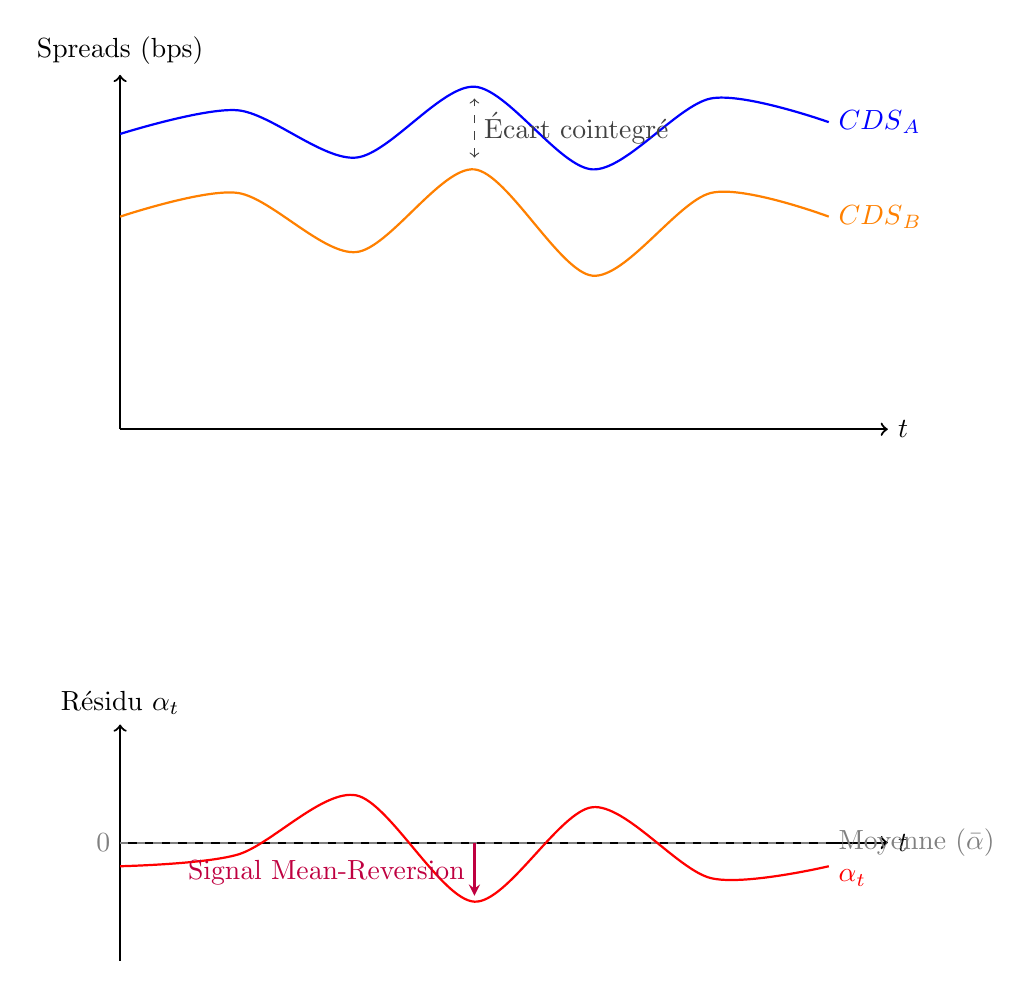
\begin{tikzpicture}[scale=1.5]
        % Repère Spread CDS A & B
        \draw[->, thick] (0, 0) -- (6.5, 0) node[right] {$t$};
        \draw[->, thick] (0, 0) -- (0, 3) node[above] {Spreads (bps)};
        
        % CDS A (exemple plus haut)
        \draw[thick, blue, smooth] plot coordinates {
            (0, 2.5) (1, 2.7) (2, 2.3) (3, 2.9) (4, 2.2) (5, 2.8) (6, 2.6)
        };
        \node[right, blue] at (6, 2.6) {$\text{CDS}_A$};
        
        % CDS B (exemple plus bas mais colinéaire)
        \draw[thick, orange, smooth] plot coordinates {
            (0, 1.8) (1, 2.0) (2, 1.5) (3, 2.2) (4, 1.3) (5, 2.0) (6, 1.8)
        };
        \node[right, orange] at (6, 1.8) {$\text{CDS}_B$};

        % Flèches de corrélation
        \draw[<->, dashed, darkgray] (3, 2.3) -- (3, 2.8);
        \node[right, darkgray] at (3, 2.55) {Écart cointegré};

        % Repère Résidu (Z-Score ou Alpha) - shifté vers le bas
        \begin{scope}[yshift=-2.5cm]
            \draw[->, thick] (0, -1) -- (6.5, -1) node[right] {$t$};
            \draw[->, thick] (0, -2) -- (0, 0) node[above] {Résidu $\alpha_t$};
            
            % Moyenne Historique
            \draw[dashed, thick, gray] (0, -1) -- (6, -1);
            \node[left, gray] at (0, -1) {$0$};
            \node[right, gray] at (6, -1) {Moyenne ($\bar{\alpha}$)};
            
            % Résidu
            \draw[thick, red, smooth] plot coordinates {
                (0, -1.2) (1, -1.1) (2, -0.6) (3, -1.5) (4, -0.7) (5, -1.3) (6, -1.2)
            };
            \node[right, red] at (6, -1.3) {$\alpha_t$};

            % Zoom sur un pic
            \draw[->, >=stealth, thick, purple] (3, -1) -- (3, -1.45);
            \node[left, purple] at (3, -1.25) {Signal Mean-Reversion};
        \end{scope}
    \end{tikzpicture}
    \caption{Pair Trading de CDS : Les deux spreads temporels cointégrés et leur résidu stationnaire ($\alpha_t = \text{CDS}_A - \beta \text{CDS}_B$)}
\end{figure}

\subsection{Défis du Trading Systématique (Frais et Liquidité)}

L'implémentation puriste algorithmique (tout systématique) d'arbitrages de Pair Trading en crédit s'affronte inéluctablement à un frein pragmatique du gré à gré (OTC) : le \textbf{coût de liquidité}. 
Parce que les marchés de crédit sont fondamentalement moins fréquents ou moins fluides que l'Action ou les FX, le "bid-ask" d'entrée décourage le trade permanent pour de ridicules signaux, dictant la sélectivité stratégique : seuls de très forts retours à la moyenne, d'assez grand horizons (Mean Reversion) justifieront un "Fair Value gap" digne d'investissement.

\section{La Base Obligation-CDS (Bond vs CDS)}

La relation théorique et l'arbitrage possible entre le marché obligataire cash (les obligations classiques) et le marché des dérivés de crédit (CDS) se matérialisent à travers l'étude de la \textbf{Base (Basis)}. 
Sur le marché, le prix d'une obligation $P$ est couramment coté en ajoutant au taux sans risque $r$ une prime de crédit et de liquidité appelée \textbf{Z-Spread} ($z$) :
\begin{equation}
    P(z) = 1 + (c - r - z) \times \frac{1 - e^{-(r+z)(T-t)}}{r+z}
\end{equation}

Toutefois, en modélisant l'obligation avec notre \textbf{intensité de défaut} ($\lambda$) et un taux de recouvrement fixé ($R$), la valorisation théorique s'écrit :
\begin{equation}
    P(\lambda) = 1 + \left(c - r - (1-R)\lambda\right) \times \frac{1 - e^{-(r+\lambda)(T-t)}}{r+\lambda}
\end{equation}

Sachant que le spread équilibré d'un CDS, $S_{\text{CDS}}$, s'approxime par $\lambda(1-R)$, il est d'usage de réécrire le prix synthétique de l'obligation en substituant l'intensité $\lambda$ par le coût de protection extrait du marché $\frac{S_{\text{CDS}}}{1-R}$ :
\begin{equation}
    P(S_{\text{CDS}}) = 1 + (c - r - S_{\text{CDS}}) \times \frac{1 - e^{-\left(r+\frac{S_{\text{CDS}}}{1-R}\right)(T-t)}}{r + \frac{S_{\text{CDS}}}{1-R}}
\end{equation}

Les traders comparent alors régulièrement la valeur du risque $S_{\text{CDS}}$ (le spread du contrat dérivé) avec la valeur théorique $\hat{S}_{\text{CDS}}(z)$ (le spread implicite déduit du prix de l'obligation cash). 
Si la différence (la \textit{Base}) s'écarte significativement de zéro, ce déséquilibre entre la composante obligataire physique et sa contrepartie dérivée ("le basis trade") génère l'opportunité d'initier conjointement un achat de l'obligation croisé à un achat de protection CDS, de sorte à arbitrer la reconstitution inhérente des primes de risque de l'entité.

\section{Performances : Carry, Roll-Down et P\&L d'un CDS}

Lorsqu'un investisseur prend une position directionnelle sur un Credit Default Swap (par exemple, une \textbf{Vente de Protection} pour s'exposer "long" au risque de crédit et toucher le spread), la performance de la position (P\&L) est influencée par l'écoulement du temps et les variations de marché.

\subsection{L'Upfront et la décomposition du P\&L}

Considérons un contrat vendu à l'instant $t_0$, de maturité $T$, avec un spread courant $S_{t_0}$ et un coupon fixe $c$. L'Upsfront (UF) initial payé ou reçu compense la différence entre le coupon et le marché :
\begin{equation}
    UF(S, c, R, r, T) = (S - c) \times PV01(S, R, r, T)
\end{equation}

Au fil du temps, disons ente $t_0$ et $t_1$, la position rapporte les coupons courants et subit une réévaluation de marché (Mark-to-Market). Le P\&L net s'écrit formellement :
\begin{equation}
    P\&L(t_0, t_1) = UF_{t_0} - UF_{t_1} + c(t_1 - t_0)
\end{equation}

Cette équation de P\&L (appliquée à la vente de protection) se décompose usuellement en se basant sur la \textit{Risky Duration} (PV01) pour isoler l'impact de chaque source de performance. En notant $\Delta t = t_1 - t_0$, les trois termes s'approximent par :
\begin{enumerate}
    \item \textbf{Carry} (impact de l'encaissement régulier du spread brut) :
    \begin{equation}
        \text{Carry} \approx S_{t_0, T} \times \Delta t
    \end{equation}
    
    \item \textbf{Roll-down} (glissement temporel de la maturité le long de la courbe des spreads initiale $t_0$, sans subir de nouveau choc de marché) :
    \begin{equation}
        \text{Roll-down} \approx \underbrace{\frac{\Delta S}{\Delta t}}_{\text{Pente}} \times \Delta t \times PV01(t_1)
    \end{equation}
    
    \item \textbf{Mark-to-Market (MtM)} (déplacement inattendu de la courbe globale des spreads de crédit entre l'instant $t_0$ et $t_1$) :
    \begin{equation}
        \text{MtM} \approx \Delta \text{Spread}_{t_0 \to t_1} \times PV01(t_1)
    \end{equation}
\end{enumerate}

\subsection{Dynamique du Roll-down et du Mark-to-Market}

\begin{figure}[H]
    \centering
    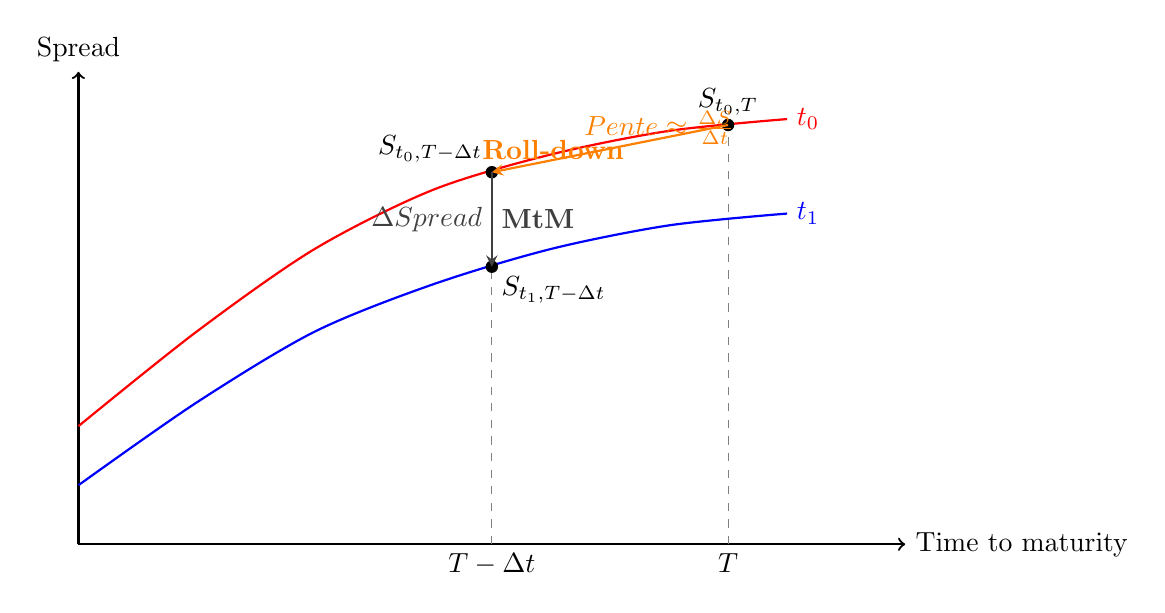
\begin{tikzpicture}[scale=1.5]
        % Axes
        \draw[->, thick] (0,0) -- (7,0) node[right] {Time to maturity};
        \draw[->, thick] (0,0) -- (0,4) node[above] {Spread};
        
        % Courbe t0 (Rouge)
        \draw[thick, red, smooth] plot coordinates {
            (0, 1.0) (1, 1.8) (2, 2.5) (3, 3.0) (4, 3.3) (5, 3.5) (6, 3.6)
        };
        \node[right, red] at (6, 3.6) {$t_0$};

        % Courbe t1 (Bleue - choquée vers le bas)
        \draw[thick, blue, smooth] plot coordinates {
            (0, 0.5) (1, 1.2) (2, 1.8) (3, 2.2) (4, 2.5) (5, 2.7) (6, 2.8)
        };
        \node[right, blue] at (6, 2.8) {$t_1$};
        
        % Positions cles
        \coordinate (T) at (5.5, 0);
        \coordinate (Tdt) at (3.5, 0);
        
        \node[below] at (T) {$T$};
        \node[below] at (Tdt) {$T - \Delta t$};
        \draw[dashed, thin, gray] (5.5, 0) -- (5.5, 3.55);
        \draw[dashed, thin, gray] (3.5, 0) -- (3.5, 3.15);
        
        % Points sur courbe t0
        \fill[black] (5.5, 3.55) circle (1.5pt) node[above] {$S_{t_0, T}$};
        \fill[black] (3.5, 3.15) circle (1.5pt) node[above left] {$S_{t_0, T-\Delta t}$};
        
        % Point sur courbe t1
        \fill[black] (3.5, 2.35) circle (1.5pt) node[below right] {$S_{t_1, T-\Delta t}$};
        
        % Fleche Roll-Down (T -> T-dt sur rouge)
        \draw[->, >=stealth, thick, orange] (5.5, 3.55) -- (3.5, 3.15);
        \node[above right, orange] at (4.2, 3.3) {$\text{Pente} \approx \frac{\Delta S}{\Delta t}$};
        \node[below left, orange] at (4.7, 3.5) {\textbf{Roll-down}};
        
        % Fleche MtM (T-dt rouge -> T-dt bleu)
        \draw[->, >=stealth, thick, darkgray] (3.5, 3.15) -- (3.5, 2.35);
        \node[left, darkgray] at (3.5, 2.75) {$\Delta \text{Spread}$};
        \node[right, darkgray] at (3.5, 2.75) {\textbf{MtM}};
    \end{tikzpicture}
    \caption{Décomposition graphique du P\&L entre le \textit{Roll-down} (glissement le long de la courbe statique) et le \textit{Mark-to-Market} (déplacement complet de la courbe)}
\end{figure}

Si la courbe de crédit ne subit aucun choc ("Mark-to-Market" nul), l'investisseur empoche non seulement le revenu du spread lié au \textbf{Carry} (ici 50 points de base / an), mais capte également la "descente" de l'instrument sur la courbe des taux. 

\textbf{Exemple} : En l'espace d'une année $t_0 \to t_1$, le contrat CDS de maturité 5 ans devient mécaniquement un CDS à 4 ans. 
Le contrat s'est revalorisé à la baisse de 50 bps à 40 bps. L'investisseur réalise un profit en revendant moins cher sa protection : le \textbf{Roll-Down}. Son gain total espéré sur l'année sera d'environ :
\begin{equation}
    P\&L(\text{statique}) \approx 50\,\text{bps} + \left( (50 - 40) \times 4\,\text{ans (PV01)} \right) = 50 + 40 = 90\,\text{bps}
\end{equation}
Les stratégies systématiques d'indices de CDS visent précisément à maximiser ce \textit{Carry Roll-down} via un "rollover" constant des séries 5 ans tous les 6 mois, tout en acceptant d'exposer le portefeuille au risque de \textbf{Mark-to-Market} en cas d'élargissement global subit de la courbe des spreads (exigences "Risk-On").
